\documentclass{article}
\usepackage{natbib}
\usepackage[labelfont=bf]{caption}
\usepackage{subcaption}
\usepackage{graphicx}
\usepackage{float}
\bibliographystyle{apalike}
\usepackage{lineno}
\linenumbers

\usepackage{geometry}
\geometry{letterpaper}
\geometry{margin=1in}

\usepackage{setspace}
\doublespacing
\captionsetup[figure]{font={stretch=2}}

\usepackage{authblk}

\newcommand{\matr}[1]{\mathbf{#1}}

\title{Application of the XT3D Multi-Point Flux Approximation to Vertically Staggered Grids in MODFLOW 6 to Improve Accuracy of Simulated Flows in Steeply Dipping Layers}
\author{
	Xt3d Enthusiast1, Affiliation1  \\
	\and 
	Xt3d Enthusiast2, Affiliation2 \\
	\and 
	Xt3d Enthusiast3, Affiliation3 \\
	\and 
	Xt3d Enthusiast4, Affiliation4 \\
	}

\date{\today}

\begin{document}

\maketitle

\textbf{Conflict of interest:} There is no conflict that is of interest to us.

\textbf{Key words:} keyboard, keynote, turnkey, turkey, monkey

\textbf{Article impact statement:} This will likely leave a sizable impact crater.

\begin{abstract}
This is the best paper ever...
\end{abstract}

\section{Introduction}

Some intro stuff here about MODFLOW \citep{modflow6framework, modflow6gwf, modflow6gwt}...

XXXXX If cell-cell flows are inaccurate, advective and dispersive transport will be inaccurate XXXXX

MODFLOW requires model cells to have horizontal tops and bottoms. In versions of MODFLOW up to and including MODFLOW-2005 \citep{modflow2005}, which offered only structured grids composed of rows, columns and layers of cells, a horizontal top and bottom allowed each cell to be ``simulated as if it were rectangular so that flow may be approximated by the standard finite-difference equation" \citep{modflow84}. In MODFLOW-USG \citep{modflowusg} and MODFLOW 6 \citep{modflow6gwf}, which offer unstructured grids and use the control-volume finite-difference method to formulate the discrete balance equations, horizontal cell tops and bottoms still simplify the definition and calculation of water-table elevations, cell saturations, and conductances between cells. In all versions of MODFLOW, cells in the same model layer can be vertically offset from each other to allow model layers to ``deform'" with the hydrostratigraphy and thereby ``minimize the number of model layers required to simulate an aquifer system" \citep{modflow84} relative to a rectilinear grid with strictly horizontal layers.

Prior to MODFLOW 6, all versions of MODFLOW used a ``conductance-based" formulation to approximate the flow between two adjacent cells. The conductance-based formulation is a ``two-point" approximation in which the flow is proportional to the difference in the heads computed at the two cell centers and a conductance that depends on the hydraulic conductivities of the cells along the direction of the cell connection, the area of the cell interface, and a measure of the distance between the cell centers. On structured MODFLOW grids with no vertical offset between cells, i.e., strictly rectilinear grids, with hydraulic conductivity that is isotropic or has anisotropy aligned with the three mutually perpendicular grid directions, the conductance-based formulation is second-order accurate \citep{dehotin2010modeling, modflow6gwf}. This is because structured MODFLOW grids with no vertical offset satisfy the ``control-volume finite-difference (CVFD) requirement" that the straight-line connection between two cell centers must intersect the midpoint of the cell interface at a right angle \citep{narasimhan1976integrated}. Structured MODFLOW grids with vertical offset between cells, which we will call "vertically offset" grids, violate the CFVD requirement because nominally "horizontal" connections between cell centers in the same layer are not strictly horizontal and therefore not perpendicular to the vertical cell interfaces they intersect. (XXXXX Also, in the grids considered by \cite{narasimhan1976integrated}, there was no partial overlap between cells faces, but is that relevant, and do we want to get into that? XXXXX) The accuracy of the conductance-based flow formulation decreases with increasing vertical offset. For this reason, the MODFLOW 6 documentation \citep{modflow6gwf} warns that "[s]teeply dipping layers generally should not be represented" using vertical offsets. \cite{anderson2015applied} recommend a $10^{\circ}$ dip as a practical upper limit for using vertical offsets. A traditional alternative to using a vertically offset grid is to map the hydrologic properties of the aquifer system onto a strictly rectilinear grid, which typically requires more model layers to adequately discretize dipping hydrostratigraphic units \citep{modflow84}.

The ability to use unstructured, or ``irregular," grids in MODFLOW-USG and MODFLOW 6 introduced the potential for grids to violate the CVFD requirement and thereby render the conductance-based formulation less accurate even in the absence of vertical offsets. To improve accuracy on irregular grids, and to allow accurate simulation of arbitrarily oriented two- or three-dimensional anisotropy, the optional XT3D flow formulation \citep{modflow6xt3d} was introduced in MODFLOW 6. XT3D formulates the flow between two cells by interpolating head values from the two cells and their neighboring cells to construct an estimate of the full, two- or three-dimensional head-gradient vector on each side of the cell interface; applying the cell conductivity tensors to obtain an estimate of the groundwater flux vector on each side of the interface; and reconciling the two flux estimates to ensure continuity of flow across the interface. By performing flow calculations using Darcy's Law in its tensorial form, based on a ``multi-point" approximation of the head gradient, XT3D accounts for both arbitrarily oriented anisotropy and geometric irregularity of the grid.

\cite{bardot2022} evaluated the effects of grid design and XT3D on the ability of MODFLOW 6 to accurately simulate flow through sedimentary structures by modeling a two-dimensional, permeable channel embedded in a nearly impermeable surrounding medium, or ``domain." The channel was angled counterclockwise from the $x$ axis of the model coordinates (by $30^{\circ}$ in most cases), and constant-head boundary conditions at the ends of the channel were set to induce uniform flow along the channel in the analytical solution. In their plan-view benchmark, the channel and surrounding domain were discretized using either a ``Regular Cartesian (RC)" grid that is rectilinear and satisfies the CVFD requirement or a ``Flexible Triangular (FT)" grid that is unstructured with triangular cells and does not satisfy the CVFD requirement. They found that the standard, conductance-based flow formulation gave accurate results on the RC grid but was subject to significant error on the FC grid, whereas the XT3D flow formulation gave accurate results on both grids, as expected. However, in their transect (cross-sectional) benchmark, which used a vertically offset grid to discretize the domain and a channel inclined by $30^{\circ}$, similarly poor results were observed with and without XT3D. The simulated groundwater flux was nearly horizontal ($0.01 - 0.03^{\circ}$ incline), and its magnitude was overestimated by 12 - 15\%. Given the ability of XT3D to compensate for violations of the CVFD requirement, it appeared likely that another aspect of the problem formulation or the inner workings of MODFLOW 6 was responsible for the unexpected results. (XXXXX Specifically mention that the NPF angle-specification "nozee" issue was looked into a found not to be the problem? Kind of an awkward detail to shoehorn in, but it would advertise this potential pitfall, which probably isn't well-known XXXXX) \cite{bardot2022} noted a suggestion by two authors of the present paper (Provost and Langevin) that inadequate grid connectivity was at the root of the problem.

"Vertically staggered" grid connections were introduced in MODFLOW-USG \citep{modflowusg} and included for the DISU grid type in MODFLOW 6 \citep{modflow6gwf} primarily as a means to vertically subdiscretize portions of a grid that is conceptualized as being layered. In a vertically staggered grid, i.e., a grid that includes vertically staggered connections, some cells have nominally ``horizontal" connections with more than one cell across a given cell face. Vertically staggered MODFLOW 6 DISU grids allow more flexibility in assigning grid connectivity than do the more commonly used DIS and DISV grid types \citep{modflow6gwf}. To our knowledge, the implications of limited grid connectivity for the accuracy of simulated flows in models with steeply dipping layers, and the potential for using vertically staggered grids to overcome this limitation, have not been previously appreciated or investigated.

In the remainder of this paper we first present a theoretical justification for the hypothesis that inadequate grid connectivity is primarily responsible for the inaccurate simulation of flows in the steeply dipping channel benchmark on a vertically offset grid. Based on that theory, we propose a method for improving the accuracy of the flow solution using XT3D together with a vertically staggered grid, and we evaluate the effectiveness of that approach in a set of benchmark problems similar to those of \cite{bardot2022}. Finally, we discuss the potential implications of our findings for practical groundwater models that include high permeability contrasts and steeply dipping layers.

XXXXX Random thoughts:
\begin{itemize}
	\item Vertical offset happens even on a completely rectilinear grid if the water table elevation varies in horizontally adjacent cells. Doesn't seem like the same kind of issue, but think on it.
	\item What happens with a head gradient perpendicular to the dip of the channel (across rather than along the channel)? Preliminary results suggest cross-connections and xt3d help.
	\item Could also try making the channel less permeable than the domain; semi-confining unit.
	\item Difference between truly single-layer model of channel vs embedded single-layer channel -- no vertical connections vs vertical connections that are no-flux. Effect on specific discharge calculations?
\end{itemize}

\section{Theoretical Background}

\begin{figure}
	\begin{center}
%	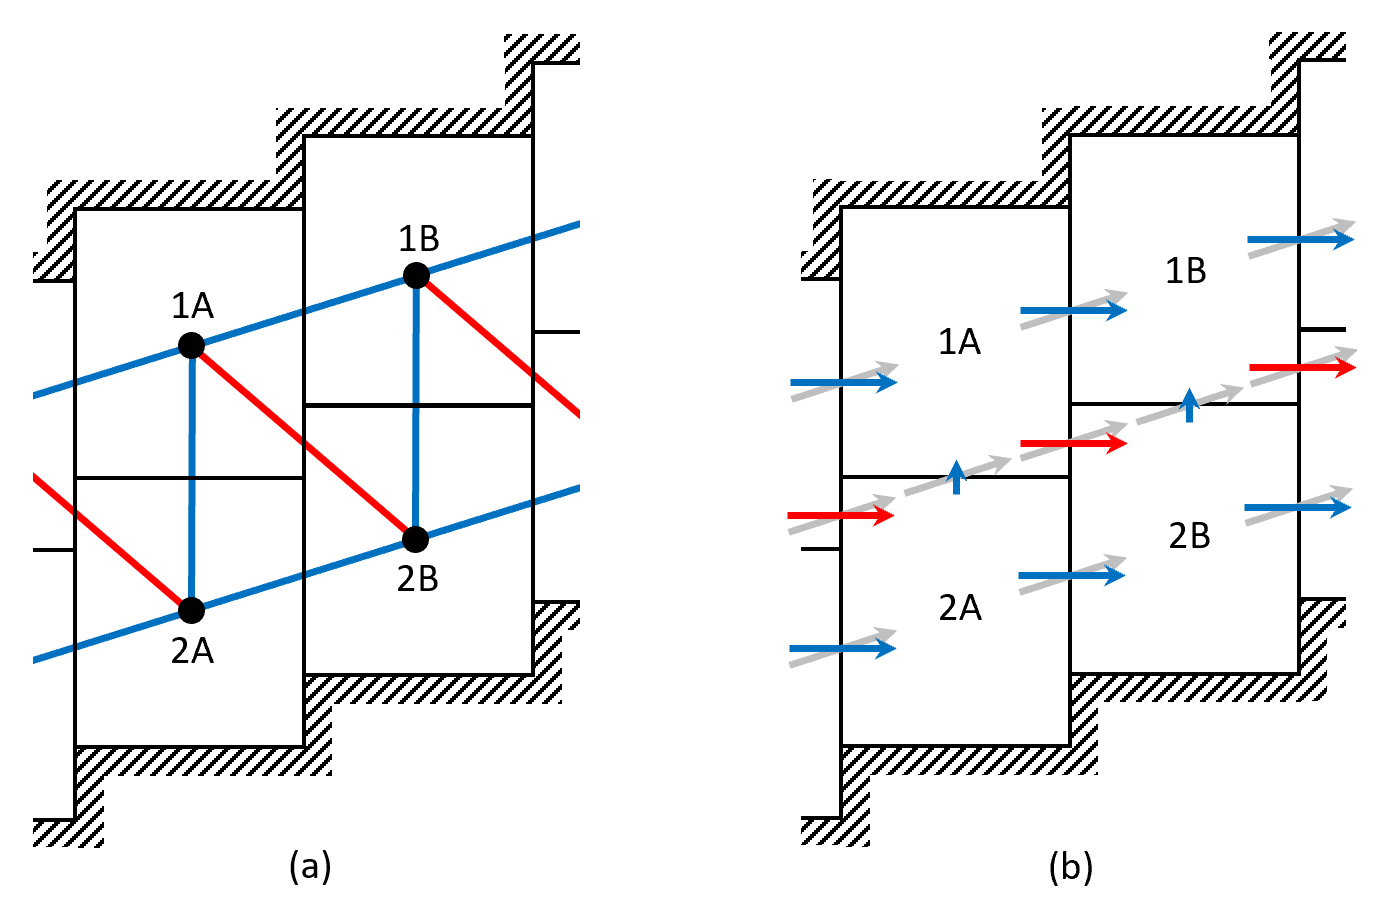
\includegraphics[scale=0.8]{../figures/schem_conn_area_flux.png}
	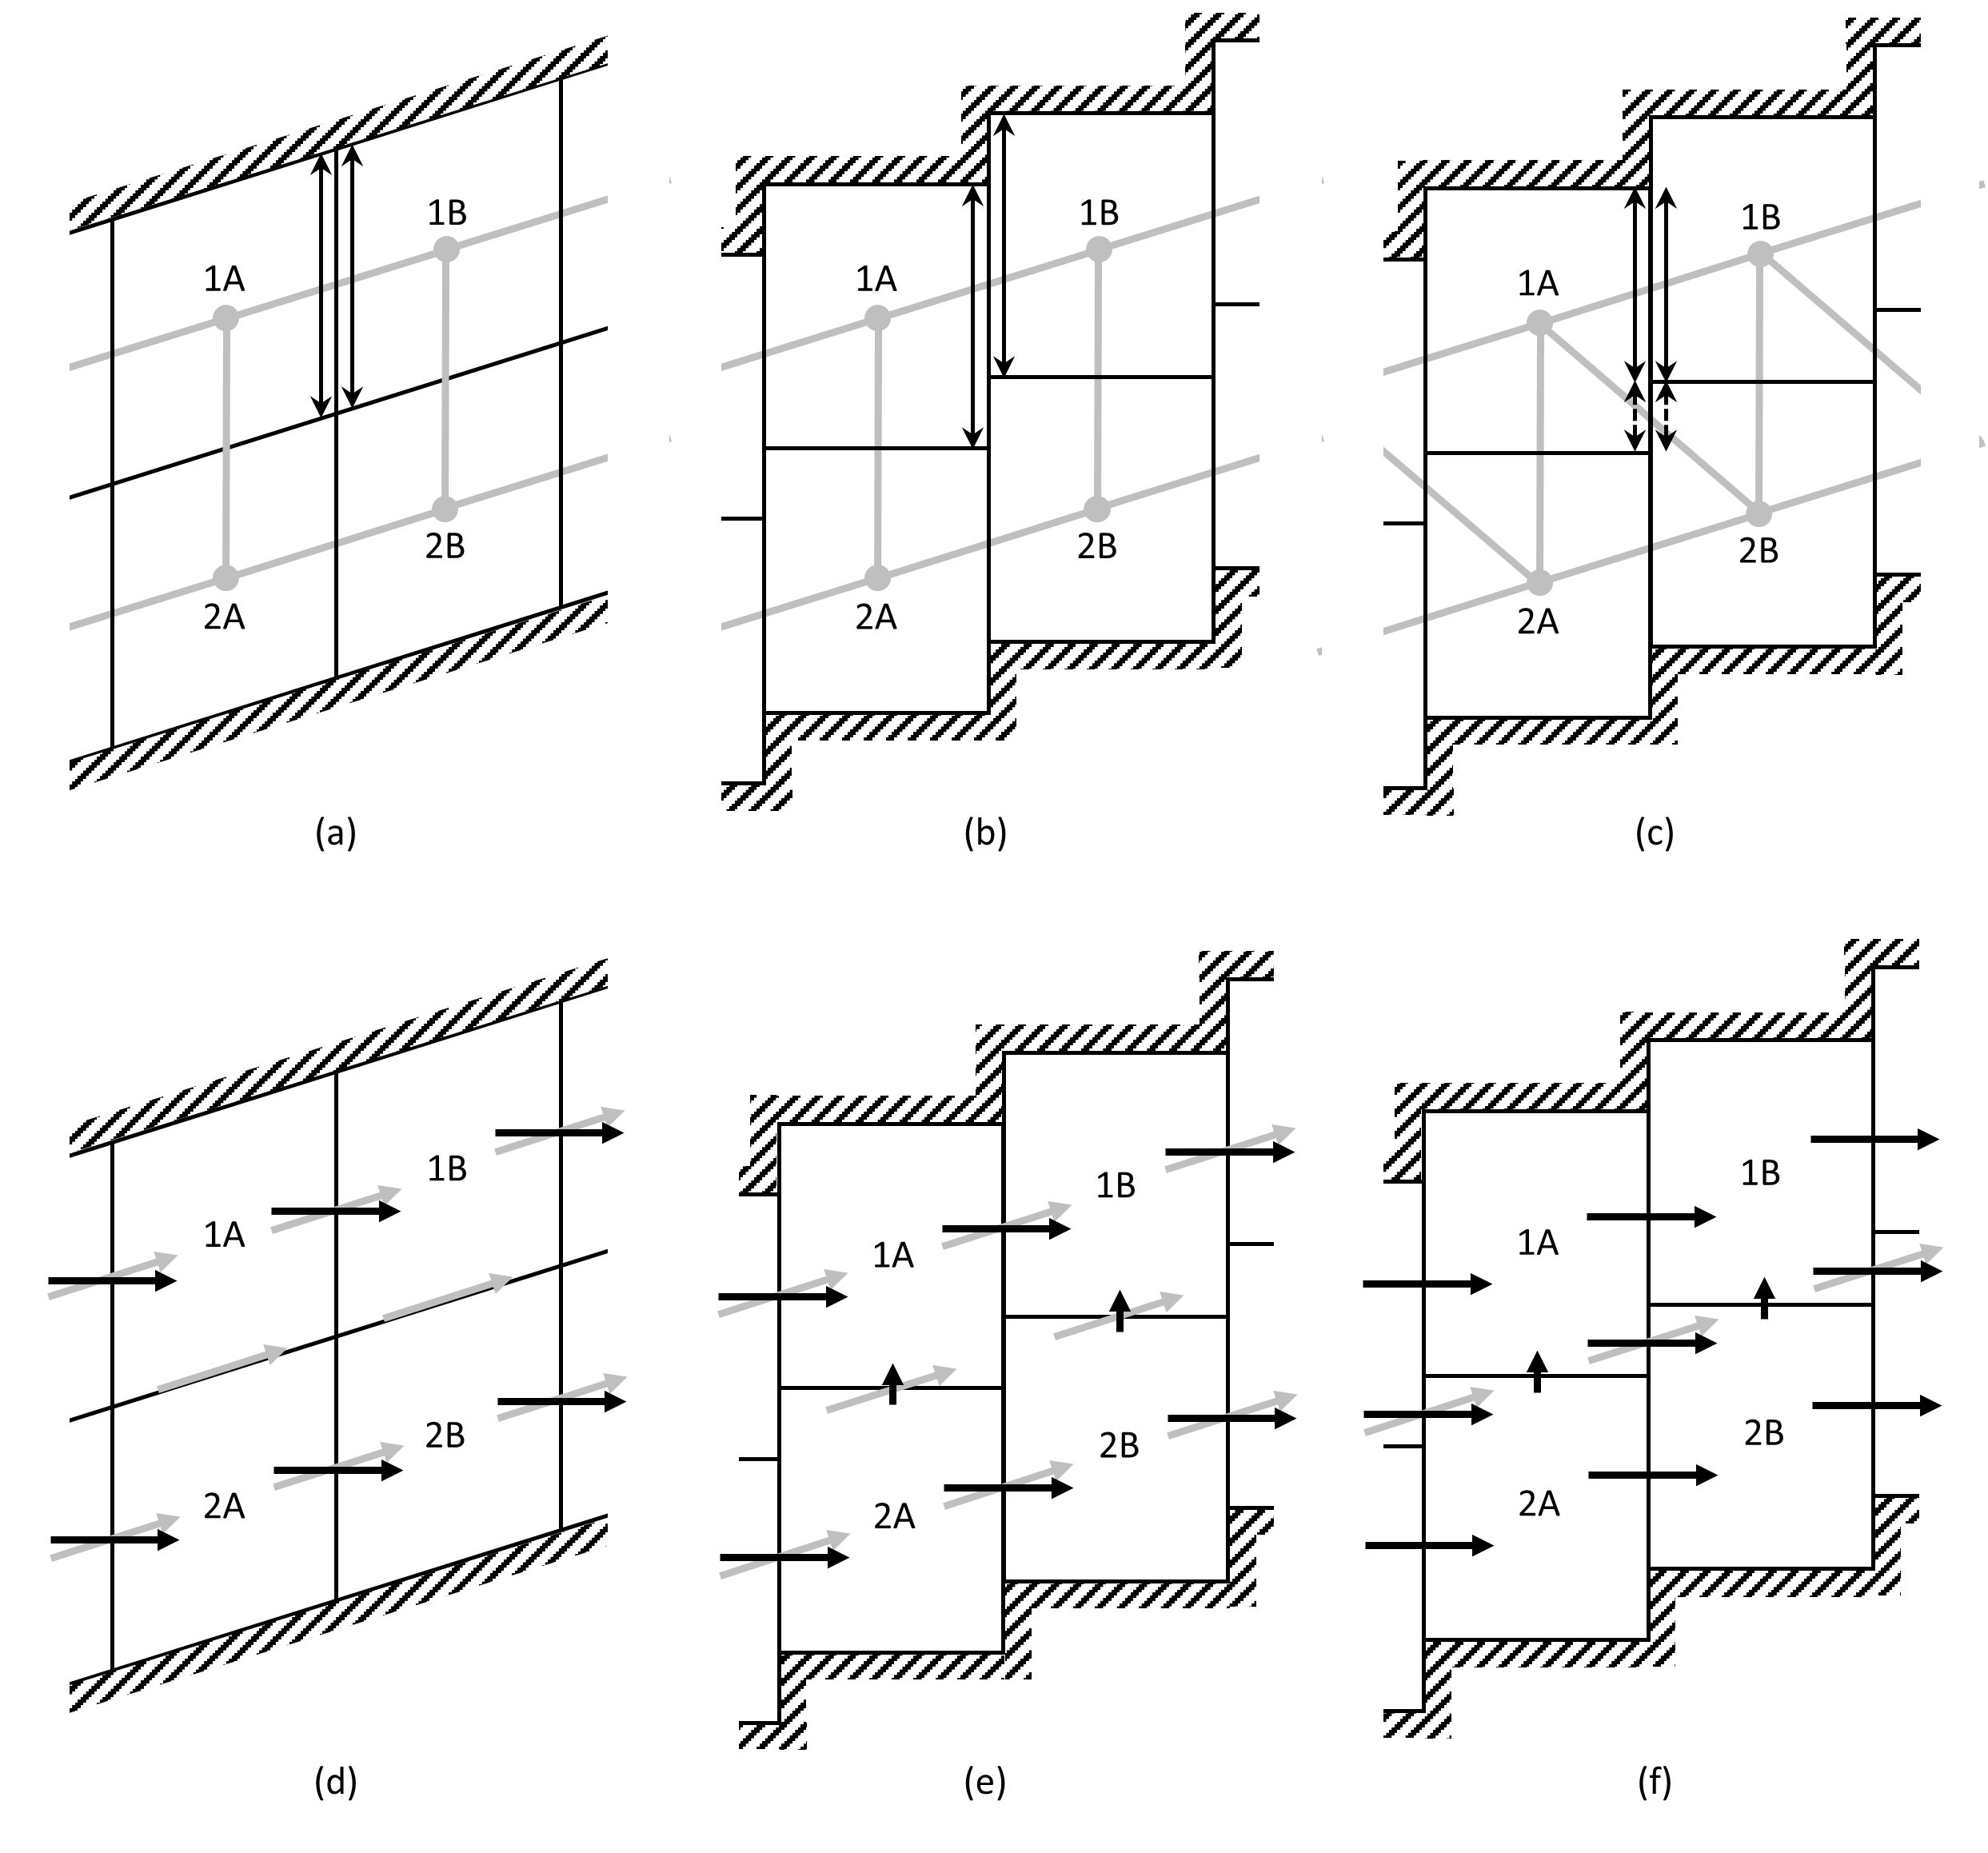
\includegraphics[scale=0.4]{../figures/schem_conn_area_flux_resaved.png}
	\caption{Schematics showing (a - c) grid connectivity and vertical cell interface areas and (c - f) cell interface fluxes in two-layer models of a dipping channel using three different grid configurations: (a, d) dip-following, (b, e) vertically offset, and (c, f) cross-connected. Hatching denotes impermeable boundaries along the top and bottom of the channel. In (a) - (c), gray circles and gray lines represent cell centers and grid connections between cells, respectively, and two-headed arrows indicate cell thicknesses used to compute cell interface areas. In (d) - (f), gray arrows represent specific-discharge (groundwater flux) vectors for uniform flow through the channel, and black arrows represent the corresponding components of flux normal to cell interfaces. For visual clarity, (f) shows gray arrows only for the cell interfaces that do not exist in (e).}
	\label{fig:schem-conn-area-flux}
	\end{center}
\end{figure}

Figure \ref{fig:schem-conn-area-flux}a shows a group of four cells in a hypothetical model in which the dipping channel is discretized vertically into two layers of cells. Although such a configuration of cells can be constructed in plan view using the DISV grid type of MODFLOW 6, it cannot be constructed in cross-section because MODFLOW requires cells to have horizontal tops and bottoms. The sloping tops and bottoms of these hypothetical cells allow the cell geometry to conform to the dip of the channel, and we will therefore refer to this grid configuration as ``dip-following." The grid connectivity is analogous to the connectivity found in a MODFLOW 6 DIS (structured, or regular) grid: a cell is hydraulically connected to each cell with which it shares a face. For example, cell 1A is connected to cells 1B and 2A, but not to cell 2B. Because cells share entire faces, i.e., adjacent cell faces overlap completely, the entire cell thickness is relevant in determining the area for flow between cells in the same layer.

One would intuitively expect a dip-following grid to be well suited to simulating uniform flow along the channel. In figure \ref{fig:schem-conn-area-flux}d, a specific discharge (groundwater flux) vector representative of uniform flow along the channel is superimposed on each cell interface, together with a vector representing the component of the flux normal to the interface. The normal flux vectors show the directions in which groundwater must be able to flow between cells to accurately represent the uniform flow field. In the case of a dip-following grid, flow must simply pass from left to right between adjacent cells in the same layer (e.g., from cell 1A to cell 1B, and from cell 2A to cell 2B). There is no flow of groundwater between cells in different layers (e.g., between cells 1A and 2A, or between cells 1B and 2B). The grid connectivity shown in figure \ref{fig:schem-conn-area-flux}a is sufficient to accommodate this straighforward pattern of flows between cells; in fact, vertical connections between cells in different layers are not even needed, and the channel could be represented just as well using a single layer.

Figure \ref{fig:schem-conn-area-flux}b shows the four cells as they would be configured for a vertically offset DIS or DISV grid in a two-layer, cross-sectional MODFLOW 6 model of the channel. The cells have horizontal tops and bottoms and can therefore follow the dip of the channel only on average, in what \cite{bardot2022} refer to as ``staircase" fashion. The pattern of grid connectivity is analogous to that in figure \ref{fig:schem-conn-area-flux}a, but it is not based strictly on which cell faces overlap. Rather, a cell is connected to each cell in the same layer with which it has an overlapping face and with each cell in an adjacent layer with which it shares a horizontal face. Significantly, cells that have overlapping vertical faces but are in different layers (e.g., cells 1A and 2B) are not connected. In the conductance-based formulation for flow, the flow between two cells in the same layer of a DIS or DISV grid (XXXXX or DISU that's not vertically staggered, but do we want to mention that here? XXXXX) is proportional to the difference in heads computed at the two cell centers and a conductance based on an effective hydraulic conductivity for the connection between the cells. If the two cells are fully saturated and have the same hydraulic conductivity and thickness, as in this example, the cell interface area used to calculate the conductance is effectively based on the full cell thickness, as shown in figure \ref{fig:schem-conn-area-flux}b. Also, the length on which the conductance is based is the horizontal distance, not the straight-line distance, between the cell centers.

As mentioned earlier, for the conductance-based flow formulation to provide maximum accuracy, the model grid must satisfy the CVFD requirement that the straight-line connection between two cell centers must intersect the midpoint of the cell interface at a right angle. In a vertically offset grid, connections between cells across vertical cell interfaces are generally not horizontal and, therefore, not perpendicular to the interface. For example, in \ref{fig:schem-conn-area-flux}b, the nominally ``horizontal" connection between cells 1A and 1B is not perpendicular to the cell interface, which compromises the accuracy of conductance-based formulations.  (XXXXX Also, in the grids considered by \cite{narasimhan1976integrated}, there was no partial overlap between cells faces, but do we want to get into that here? XXXXX)

XXXXX Mostly covered in intro, so condense here XXXXX In their dipping-channel benchmark problem, \cite{bardot2022} found that, as expected, the standard, conductance-based formulation gave poor results for a steeply dipping channel discretized using a vertically offset grid. The simulated groundwater flux in the middle of the channel was not along the $30^{\circ}$ incline of the channel, but nearly horizontal ($0.03^{\circ}$ incline), and its magnitude was overestimated by 15\%. Given the ability of XT3D to compensate for grid connections that are not perpendicular to cell interfaces, rerunning the simulation with XT3D activated could have been expected to improve the flow solution substantially. However, \cite{bardot2022} observed similarly poor results with XT3D: the flux was still nearly horizontal ($0.01^{\circ}$ incline), and its magnitude was overestimated by 12\%. Something other than a simple violation of the CVFD perpendicularity condition was evidently responsible, and \cite{bardot2022} noted a suggestion by two authors of the present paper (Provost and Langevin) that inadequate grid connectivity was at the root of the problem.

The influence of grid connectivity on the results observed by \cite{bardot2022} can be explained with the help of figures \ref{fig:schem-conn-area-flux}b and \ref{fig:schem-conn-area-flux}e. Figure \ref{fig:schem-conn-area-flux}e shows the specific discharge vector superimposed on each cell interface of the vertically offset grid, together with a vector representing the component of the flux normal to the interface. As in the case of a dip-following grid (figure \ref{fig:schem-conn-area-flux}d), flow passes from left to right between adjacent cells in the same layer. However, unlike in the dip-following grid, there must also be vertical flow from each cell in layer 2 and to the cell immediately above it in layer 1 (e.g., from cell 2A and to cell 1A). This pattern of flow between cells obviously cannot be a solution to uniform, steady-state flow through the channel, since the exclusively upward vertical flows would deplete layer 2 and accumulate water in layer 1. Short of resorting to alternating upward and downward vertical flows, which would compromise the uniformity of the flow, the only alternative for representing uniform, steady-state flow on the vertically offset grid is to have exclusively horizontal flow. Although this concept is illustrated for a two-layer model in figure \ref{fig:schem-conn-area-flux}e, the same reasoning applies to a model of the channel with any number of layers. This explains why \cite{bardot2022} observed nearly horizontal flow in the middle portion of the channel, away from the lateral boundaries, where nearly uniform flow was established. Thus, it appears the nearly horizontal flows are not primarily due to what \cite{bardot2022} call the ``cosine error" associated with the orientation and length of the sloping grid connections, but to the inability of the vertically offset grid to route flow appropriately between cells.

This suggests an approach for constructing the grid to improve the accuracy of the flow solution. Figure \ref{fig:schem-conn-area-flux}c shows a grid that includes additional connections between cells in different layers compared to the grid in \ref{fig:schem-conn-area-flux}b. For example, cell 1A is connected not only cells 2A and 1B, but also the cell 2B. The grid connectivity is determined by overlap between cell faces; if two cells have faces that overlap even partially, the cells are connected across those faces. The area of the interface is the area of overlap between the cell faces. This grid configuration, which was introduced MODFLOW-USG \citep{modflowusg} and is available for the DISU grid type in MODFLOW 6, is called ``vertically staggered" and allows a cell to have nominally ``horizontal" connections with more than one cell across a given cell face. In this case, vertical staggering is used to introduce ``cross-connections" between cells in different layers. The ramifications of cross-connections for flow between cells are illustrated in figure \ref{fig:schem-conn-area-flux}f. Inclusion of cross-connections (e.g., between cells 1A and 2B) allows upward vertical flows from layer 2 to layer 1 (e.g., from cell 2A to cell 1A) to be routed back down to layer 2 so water does not accumulate in layer 1. The remainder of this paper describes test problems that evaluate the effectiveness of cross-connections for improving the accuracy of simulated flow though the channel.

\section{Description of Test Problems}

The test problems are patterned after the cross-sectional (transect) benchmarks of \cite{bardot2022}. They attempt simulate uniform flow in a permeable channel embedded in a less permeable surrounding ``domain." The channel is of uniform width and hydraulic conductivity and is inclined relative to the horizontal.

To simulate flow along a channel inclined at angle $\theta$, heads are specified at the centers of cells along the perimeter of the model (XXXXX this assumes we're using the transect\_benchmark version of the model, which includes the "domain," for all of our final runs XXXXX) using an analytical solution that corresponds to a unit head gradient inclined at angle $\theta$ \citep{bardot2022}:

\begin{equation}
\label{eqn:head_analyt_along}
h = - x \cos \theta - z \sin \theta.
\end{equation}

\noindent where $h$ is head in meters and $x$ and $z$ are the horizontal and vertical model coordinates, respectively, in meters. Flow across the channel (XXXXX seems like this would be good to include XXXXX) is simulated using the modified head function
\begin{equation}
\label{eqn:head_analyt_across}
h = x \sin \theta - z \cos \theta,
\end{equation}
which represents a unit head gradient perpendicular to the long axis of the channel. In both cases, the hydraulic conductivity of the channel is set to 1 m/d (meter per day) so that the analytical flow solution is a groundwater flux of 1 m/d either along or across the channel. The conductivity of the domain surrounding the channel varies according to the scenario being investigated. In the homogeneous limit, the conductivity of the domain is set equal to that of the channel. In the highly heterogeneous limit, the conductivity of the domain is set much lower than that of the channel to effectively isolate the channel hydraulically. XXXXX Could also try making the channel less permeable than the domain; semi-confining unit XXXXX

Simulations are performed using variations on two test problems that differ in their method of discretization. The first test problem uses the traditional approach of representing the inclined channel using a vertically offset grid of the MODFLOW 6 DIS (structured) type. (XXXXX To be decided: present results for the DIS grid, or for the equivalent of the DIS grid after conversion to DISU? XXXXX) This problem confirms the findings of \cite{bardot2022} and illustrates the limitations of the vertically offset grid approach. The second test problem is similar to the first but uses a vertically staggered grid of MODFLOW 6 DISU (unstructured) type. The second problem is designed to evaluate the effectiveness of cross-connections between layers (illustrated in figure \ref{fig:schem-conn-area-flux}c) in improving the accuracy of the flow solution, both with and without XT3D. Variations on both test problems are described in the ``Results and Discussion" section.

Jupyter notebooks for both test problems are available in the Supporting Information that accompanies this paper. The notebooks leverage the capabilities of FloPy \citep{bakker2016scripting} to assist in setting up input for and processing results from the MODFLOW 6 simulations. The second test problem is formulated by starting with a DIS grid, converting it to an equivalent DISU grid, and adding cross-connections. A Python script for converting and modifying the grid is included.

\section{Results and Discussion}

XXXXX See the temporary ``preliminary results" section at the end of the manuscript XXXXX

XXXXX Results without the domain are presented first to "cleanly" illustrate the main problem and its solution. Results with the domain are then presented to give more of an indication of how things might work in practice. Unless stated otherwise, the domain is 6 orders of magnitude less conductive than the channel, as in \cite{bardot2022}. XXXXX

\subsection{Test Problem 1: Vertically Offset Discretization}

\begin{figure}[H]
\centering
\begin{subfigure}{0.4\textwidth}
	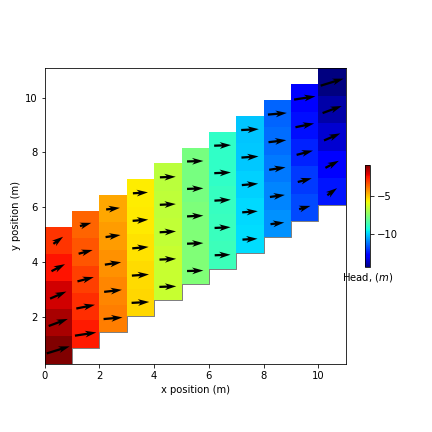
\includegraphics[width=\textwidth]{../figures/disu-af-vo-s-head.png}
	\caption{standard conductance-based formulation}
	\label{fig:disu-s-nocc-head}
\end{subfigure}
\hfill
\begin{subfigure}{0.4\textwidth}
	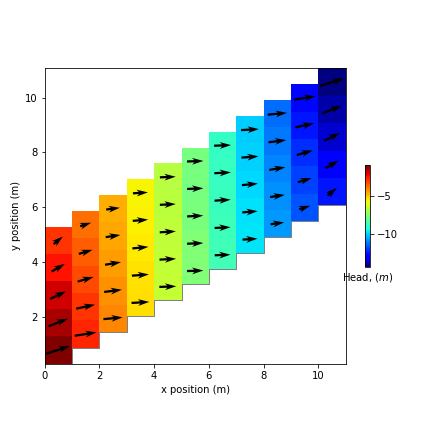
\includegraphics[width=\textwidth]{../figures/disu-af-vo-x-head.png}
	\caption{XT3D}
	\label{fig:disu-x-nocc-head}
\end{subfigure}
\caption{Specific discharge and head for a vertically offset grid. As Kerry and Jim found previously, the news is all bad; the flow tends to go horizontal, and XT3D doesn't really help. (preliminary result from disu\_approach model, 5x11 grid without cross-connections, $30^{\circ}$ incline, set up for flow along the channel; scenarios disu-af-vo-s and disu-af-vo-x)}
\label{fig:figures}
\end{figure}

\begin{figure}[H]
\centering
\begin{subfigure}{0.4\textwidth}
	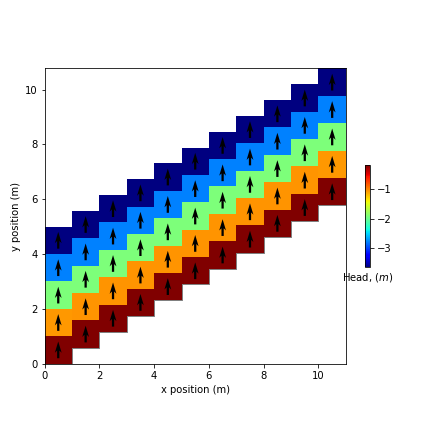
\includegraphics[width=\textwidth]{../figures/disu-cf-vo-s-head.png}
	\caption{standard conductance-based formulation}
	\label{fig:disu-s-nocc-cf-head.}
\end{subfigure}
\hfill
\begin{subfigure}{0.4\textwidth}
	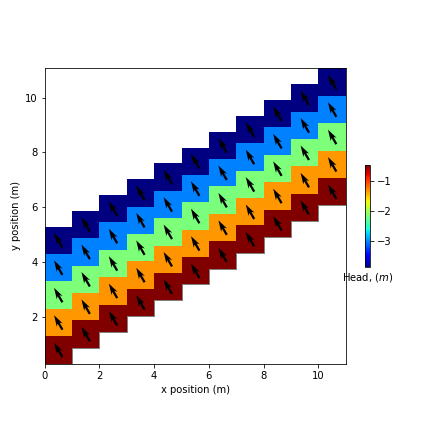
\includegraphics[width=\textwidth]{../figures/disu-cf-vo-x-head.png}
	\caption{XT3D}
	\label{fig:disu-x-nocc-cf-head}
\end{subfigure}
\caption{Specific discharge and head for a vertically offset grid and boundary heads set up for crossflow. The standard formulation is a fail, but XT3D nails it, even without cross-connections. (preliminary result from disu\_approach model, 5x11 grid without cross-connections, $30^{\circ}$ incline, set up for flow across the channel; scenarios disu-cf-vo-s and disu-cf-vo-x)}
\label{fig:figures}
\end{figure}

\subsection{Test Problem 2: Vertically Staggered Discretization}

\begin{figure}[H]
\centering
\begin{subfigure}{0.4\textwidth}
	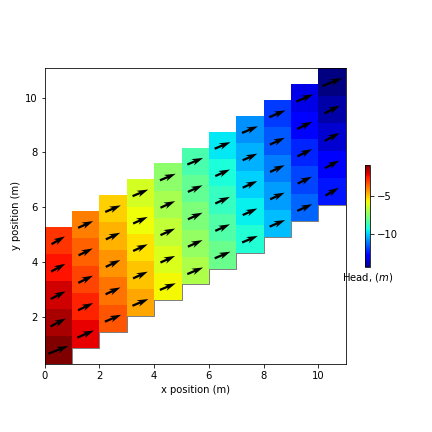
\includegraphics[width=\textwidth]{../figures/disu-af-vs-s-head.png}
	\caption{standard conductance-based formulation}
	\label{fig:disu-s-cc-head}
\end{subfigure}
\hfill
\begin{subfigure}{0.4\textwidth}
	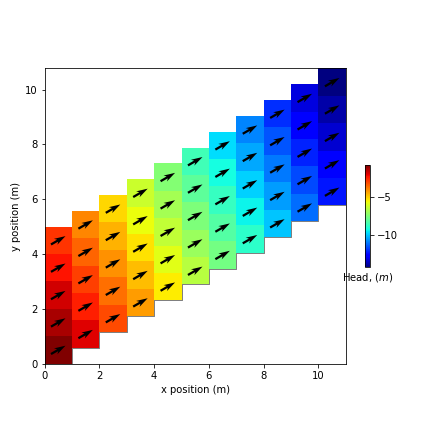
\includegraphics[width=\textwidth]{../figures/disu-af-vs-x-head.png}
	\caption{XT3D}
	\label{fig:disu-x-cc-head}
\end{subfigure}
\caption{Specific discharge and head for a vertically staggered grid with cross-connections. The news is much better; the standard formulation is much improved, and XT3D nails it. (preliminary result from disu\_approach model, 5x11 grid with cross-connections, $30^{\circ}$ incline, set up for flow along the channel; scenarios disu-af-vs-s and disu-af-vs-x)}
\label{fig:figures}
\end{figure}

\begin{figure}[H]
\centering
\begin{subfigure}{0.4\textwidth}
	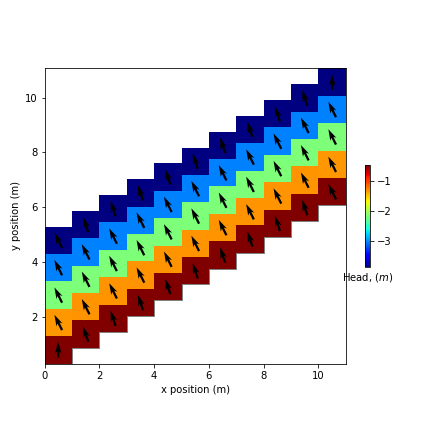
\includegraphics[width=\textwidth]{../figures/disu-cf-vs-s-head.png}
	\caption{standard conductance-based formulation}
	\label{fig:disu-s-cc-cf-head}
\end{subfigure}
\hfill
\begin{subfigure}{0.4\textwidth}
	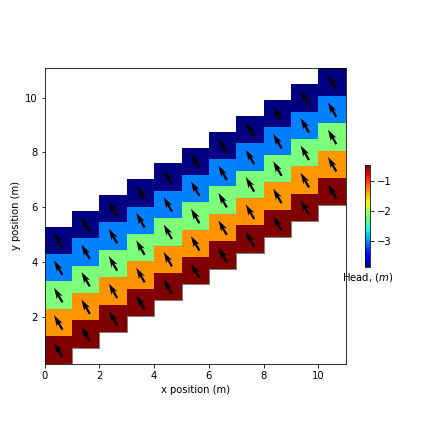
\includegraphics[width=\textwidth]{../figures/disu-cf-vs-x-head.png}
	\caption{XT3D}
	\label{fig:disu-x-cc-cf-head}
\end{subfigure}
\caption{Specific discharge and head for a vertically staggered grid with cross-connections and boundary heads set up for crossflow. The standard formulation does pretty well, and XT3D nails it. (preliminary result from disu\_approach model, 5x11 grid with cross-connections, $30^{\circ}$ incline, set up for flow across the channel; scenarios disu-cf-vs-s and disu-cf-vs-x)}
\label{fig:figures}
\end{figure}

\subsection{Test Problem 3: Vertically Offset Discretization with Domain}

\begin{figure}[H]
\centering
\begin{subfigure}{0.4\textwidth}
	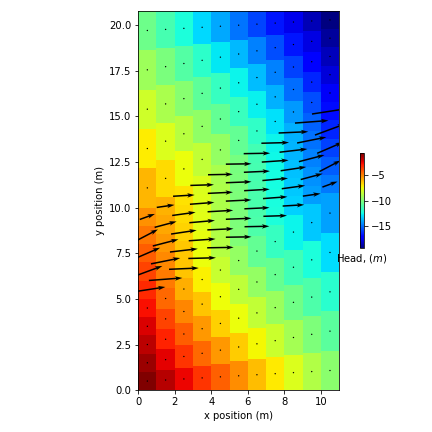
\includegraphics[width=\textwidth]{../figures/disu-d-af-vo-s-head.png}
	\caption{standard conductance-based formulation}
	\label{fig:disu-s-nocc-head}
\end{subfigure}
\hfill
\begin{subfigure}{0.4\textwidth}
	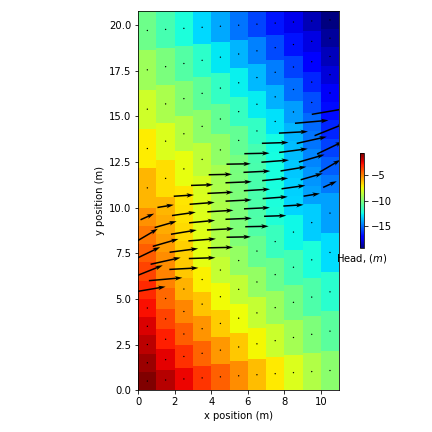
\includegraphics[width=\textwidth]{../figures/disu-d-af-vo-x-head.png}
	\caption{XT3D}
	\label{fig:disu-x-nocc-head}
\end{subfigure}
\caption{Specific discharge and head for a vertically offset grid with the domain. Results are similar to those without the domain and consistent with what Kerry and Jim found previously; the flow tends to go horizontal, and XT3D doesn't really help. (preliminary result from disu\_approach model, 5x11 channel with 5x11 subdomains above and below, without cross-connections, $30^{\circ}$ incline, set up for flow along the channel; scenarios disu-d-af-vo-s and disu-d-af-vo-x)}
\label{fig:figures}
\end{figure}

XXXXX Idea: See how heterogeneity affects the error -- series of runs with varying permeability contrast between channel and surrounding domain (from 1:1 to very large), producing a plot along the lines of figs. 3d and 4d in \cite{bardot2022}. Will need to use the transect\_benchmark model for this, as we probably should for all of the final simulations. XXXXX

\begin{figure}[H]
\centering
\begin{subfigure}{0.4\textwidth}
	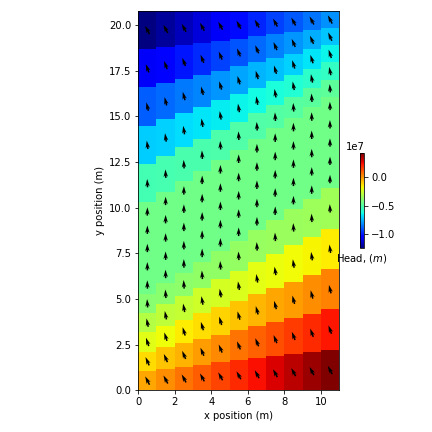
\includegraphics[width=\textwidth]{../figures/disu-d-cf-vo-s-head.png}
	\caption{standard conductance-based formulation}
	\label{fig:disu-s-nocc-cf-head.}
\end{subfigure}
\hfill
\begin{subfigure}{0.4\textwidth}
	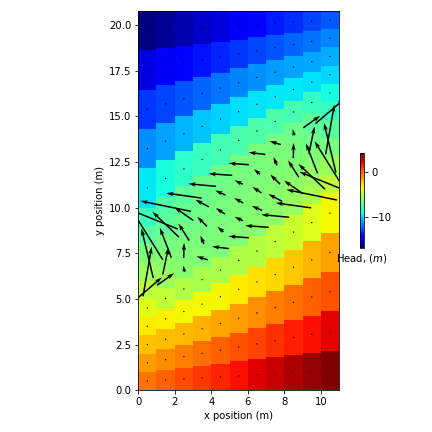
\includegraphics[width=\textwidth]{../figures/disu-d-cf-vo-x-head.png}
	\caption{XT3D}
	\label{fig:disu-x-nocc-cf-head}
\end{subfigure}
\caption{Specific discharge and head for a vertically offset grid with the domain and boundary heads set up for crossflow. The standard formulation gives nearly vertical flow in the channel, and XT3D also does poorly, even mid-channel. The huge specific discharge vectors near the channel boundary are apparently caused by XT3D's head-gradient interpolation drawing heads from the domain, where the head gradient is huge, when computing nominally horizontal flows between cells within the channel. (preliminary result from disu\_approach model, 5x11 channel with 5x11 subdomains above and below, without cross-connections, $30^{\circ}$ incline, set up for flow across the channel; scenarios disu-d-cf-vo-s and disu-d-cf-vo-x)}
\label{fig:figures}
\end{figure}

\subsection{Test Problem 4: Vertically Staggered Discretization with Domain}

\begin{figure}[H]
\centering
\begin{subfigure}{0.4\textwidth}
	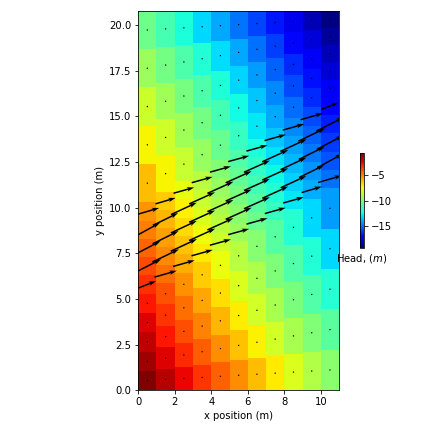
\includegraphics[width=\textwidth]{../figures/disu-d-af-vs-s-head.png}
	\caption{standard conductance-based formulation}
	\label{fig:disu-s-cc-head}
\end{subfigure}
\hfill
\begin{subfigure}{0.4\textwidth}
	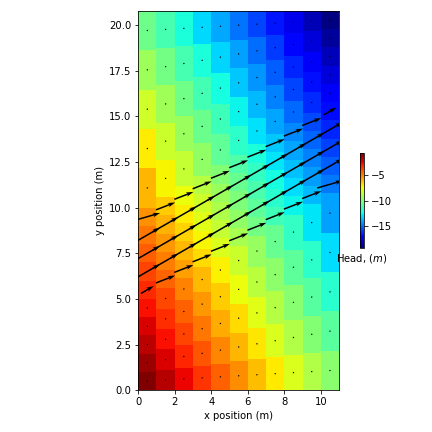
\includegraphics[width=\textwidth]{../figures/disu-d-af-vs-x-head.png}
	\caption{XT3D}
	\label{fig:disu-x-cc-head}
\end{subfigure}
\caption{Specific discharge and head for a vertically staggered grid with the domain and with cross-connections. The standard formulation isn't horrible, and XT3D does very well except at the channel boundary, where there's presumably a "staircase" effect. (preliminary result from disu\_approach model, 5x11 channel with 5x11 subdomains above and below, with cross-connections, $30^{\circ}$ incline, set up for flow along the channel; scenarios disu-d-af-vs-s and disu-d-af-vs-x)}
\label{fig:figures}
\end{figure}

\begin{figure}[H]
\centering
\begin{subfigure}{0.4\textwidth}
	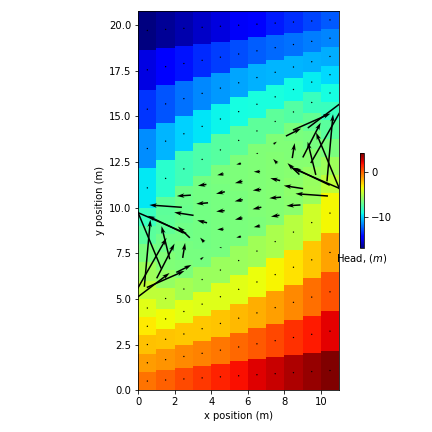
\includegraphics[width=\textwidth]{../figures/disu-d-cf-vs-s-head.png}
	\caption{standard conductance-based formulation}
	\label{fig:disu-s-cc-cf-head}
\end{subfigure}
\hfill
\begin{subfigure}{0.4\textwidth}
	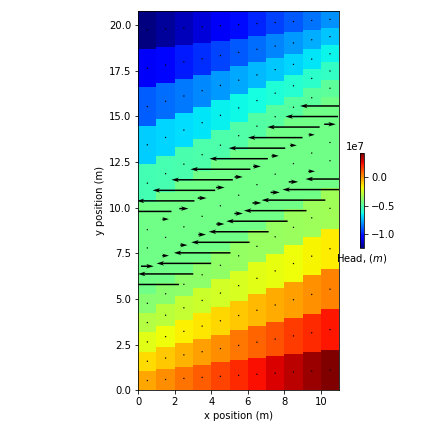
\includegraphics[width=\textwidth]{../figures/disu-d-cf-vs-x-head.png}
	\caption{XT3D}
	\label{fig:disu-x-cc-cf-head}
\end{subfigure}
\caption{Specific discharge and head for a vertically staggered grid with the domain and with cross-connections and boundary heads set up for crossflow. The standard formulation is much improved. You can't tell because of the scale of the vectors, but XT3D does well mid-channel. However, near the channel boundary it still has huge flows due to interpolating heads from the domain. (preliminary result from disu\_approach model, 5x11 channel with 5x11 subdomains above and below, $30^{\circ}$ incline, set up for flow across the channel; scenarios disu-d-cf-vs-s and disu-d-cf-vs-x)}
\label{fig:figures}
\end{figure}

\section{Conclusions}

XXXXX The concepts in this paper have been easiest to discuss in terms of layers, but they're not limited to layered grids. XXXXX

\section{Acknowledgments}
Thank all those reviewers.

\section{Supporting Information}

\section{Appendix}

\bibliography{references.bib}

\section{Oblique reference}

\begin{figure}[H]
	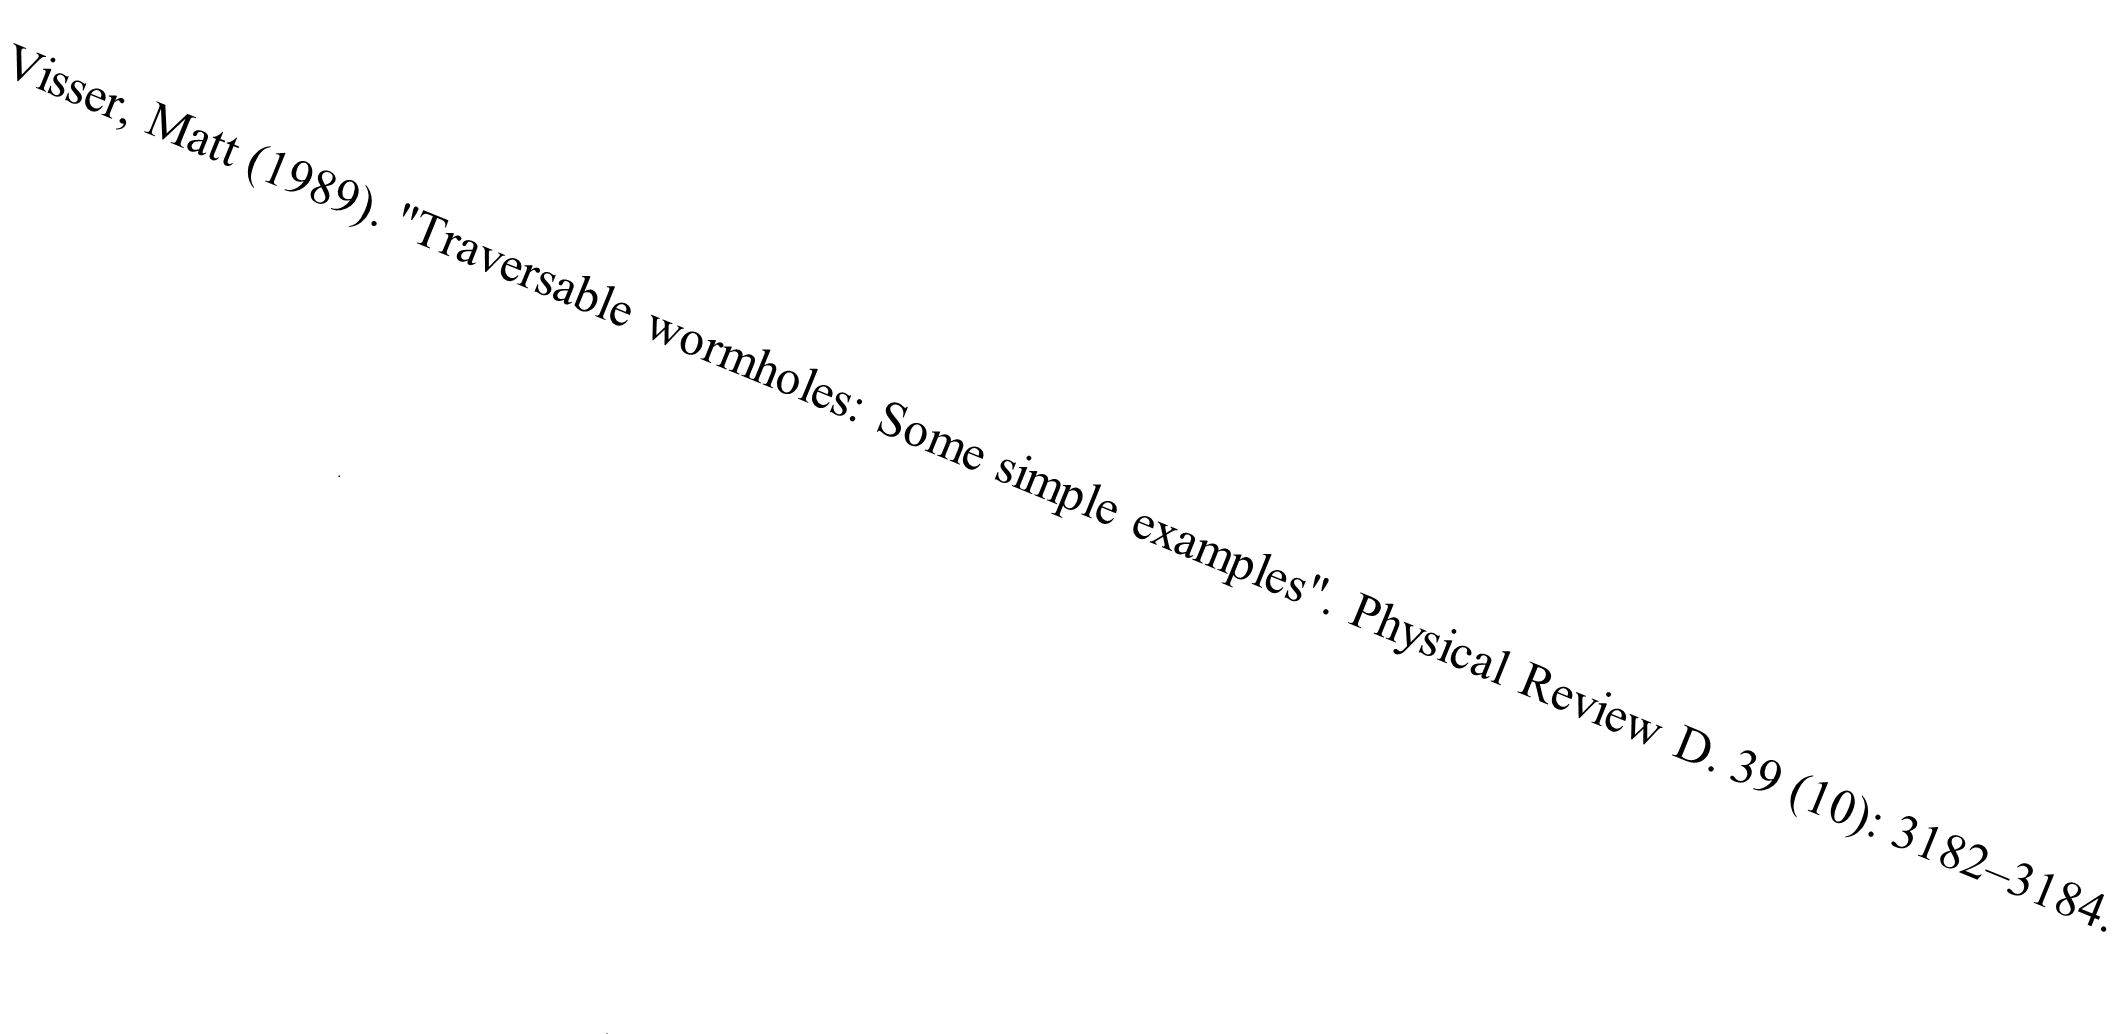
\includegraphics[scale=0.5]{../figures/oblique_reference.png}
\end{figure}

\section{preliminary results}
This temporary section is a summary of preliminary results that can help provide context and guide our thinking as we construct the story.  Specific results may or may not make it into the paper.

The models referenced are:
\begin{itemize}
	\item wormholes -- This is a plan-view, DISV model that emulates a cross-sectional model and includes ``connector" cells that can have sloped tops and bottoms. Cell dimensions and hydraulic conductivities can be adjusted to approach a ``dip-following" mesh (in which cell tops and bottoms follow the dip of the channel) at one extreme and a vertically offset mesh (the kind MODFLOW actually uses in cross-section) at another extreme. A vertically offset mesh is approached by making the width of the connector cells very small in the x direction and, in the case of xt3d, making them anisotropic with very high K (1000 x the base K in these runs) along the slope of the cell and very low K (0.001 x the base K) perpendicular to the slope. The case of a vertically offset mesh using the standard formulation, which cannot implement such anisotropy, was run but is not generally of interest. This model is in the repo, but results from this model probably won't be included in the paper.
	\item crossconnected -- This is a plan-view, DISV model that emulates a cross-sectional model with ``cross-connections" between model layers. This model is not in the repo, and results are noted here primarily to confirm the expected agreement with the disu\_approach model.
	\item disu\_approach -- This implements cross-connections ``for real" in a cross-sectional, DISU model. Specific discharge is recalculated in the notebook to account for overlap areas; the recent ``patch" to MF6 is not being used (yet).
	\item transect\_benchmark -- This is the vertically offset model of \cite{bardot2022} updated to allow cross-connections. Results from this model are not summarized here yet.
\end{itemize}

In the model of \cite{bardot2022} and its transect\_benchmark update, the channel is embedded in a surrounding ``domain."  In each of the other three models, there is no surrounding domain -- the channel is the entire model. The distinction may be significant because the surrounding matrix provides vertical connections to the channel. When the surrounding domain is (effectively) impermeable, these vertical connections contribute ``zero vertical flux" information to the specific discharge calculation, implying that the specific discharge is literally horizontal. In the absence of a surrounding domain, there is no vertical flux component information. Need to check what difference this might make.

In the plan-view models, rows function as ``layers." Unless stated otherwise, all results are for a 30-degree channel dip, and the analytical solution is a specific discharge of 1. inclined at 30 degrees. Total flow is the sum of the flows reported for the CHD cells along the left end of the channel. Numerical results are rounded arbitrarily. The terms ``specific discharge" and ``flux" are using interchangeably.

\subsection{Single-layer channel}
The channel is represented using a single layer of cells.

\subsubsection{wormholes, 1x11 cells:}
Results were the same whether the mesh was vertically offset (xt3d and standard, though not sure if standard results are meaningful) or dip-following (xt3d and standard), which is not surprising since there are no connections across the tops and bottoms. The errors in computed heads were miniscule in all cases.

\paragraph{with xt3d:} Specific discharge is 0.8660 and ``seemingly" horizontal. This makes sense if you consider that the only connections in the model are ``horizontal" ones along the layer. A horizontal flux component of 0.8660 corresponds (via the cosine factor) to a unit flux from left to right along the dip of the channel, so in that sense it's correct. Furthermore, that's the only flux component that exists in this model, and therefore the only one xt3d can calculate; the vertical flux component is reported as zero by default. So rather than say the flux is horizontal, perhaps it's fairer to say MODFLOW gets the horizontal component right and simply can't tell us what the vertical component is. Total flow is 0.8660, which is correct.

\paragraph{without xt3d (standard formulation)} Specific discharge is 1.1547 and, again, ``seemingly" horizontal. This increase in magnitude relative to xt3d makes sense because the standard formulation ignores both the angle of the connection relative to the vertical cell interface and the reduction in area for flow (area perpendicular to the long axis of the channel) when the channel dips. Therefore, the  magnitude differs by a factor of $1/{(cosine factor)}^2$. Total flow is 1.1547, which reflects the error in the flux.

\subsubsection{crossconnected, 1x11 cells:} Specific discharge results are essentially identical to those in the vertically offset wormholes model, which is not surprising given that there can be no cross-connections in a single-layer model. The errors in computed heads were miniscule with and without xt3d.

\paragraph{with xt3d:} Total flow is 0.3660, which reflects the smaller area available for flow between two cells (the overlap area).

\paragraph{without xt3d (standard formulation)} Total flow is 0.4880, which (given the incorrect flux) also reflects the smaller area available for flow between two cells (the overlap area).

\subsubsection{disu\_approach, 1x11 cells:} Specific discharge results are essentially identical to those in the vertically offset wormholes model and crossconnected model. Total flow matched either the vertically offset wormholes result or the crossconnected result depending on how the ``staggered" flag was set in the notebook, which determined whether the specific discharge remained based on average areas or was recalculated using overlap areas. (There are no cross-connections in a single-layer model, so the cell-cell flows were unaffected, so it was just a matter of whether the fluxes were postprocessed to adjust the areas.) The errors in computed heads were miniscule with and without xt3d.

\subsection{Two-layer channel}
The channel is represented using two layers of cells. This introduces the possibility of vertical flows between layers.

\subsubsection{wormholes, 2x11 cells}

\paragraph{dip-following mesh with xt3d:} In the connector cells (which are of primary interest in this case), specific discharge is 0.9998 mid-channel and 1.00003 on average, with a max error of +0.0003. Angle of specific discharge is 29.9913 deg mid-channel and 29.9879 on average, with a max error of +0.03 deg. Errors in computed heads (including all cells) are on the order of 0.002\%. Total flow is 1.7321 (0.8661 per cell). So, good agreement with the analytical solution.

\paragraph{dip-following mesh without xt3d (standard formulation)} In the connector cells (which are of primary interest in this case), specific discharge is 1.3336 mid-channel and 1.3687 on average, with a max error of +0.69. Angle of specific discharge is 30.05 deg mid-channel and 32.24 on average, with a max error of +9.8 deg. Errors in computed heads (including all cells) are on the order of 2\%. Total flow is 2.3094 (1.1547 per cell).

\paragraph{vertically offset mesh with xt3d:} In the flat-top cells (which are of primary interest in this case), specific discharge is 1.1117 mid-channel and 1.1211 on average, with a max error of +0.35. Angle of specific discharge is -0.53 deg mid-channel and 6.0095 on average, with a max error of -30.54 deg; the flow generally skews toward horizontal. Errors in computed heads (including all cells) are on the order of 4\%. Total flow is 2.1993 (1.0997 per cell).

\subsubsection{crossconnected, 2x11 cells:}

\paragraph{with xt3d:} Specific discharge matches the analytical solution very closely, with a max error of -5e-9. Angle of specific discharge also matches very closely, with a max error of -9e-8 deg. Errors in computed heads are minscule. Total flow is 1.2321 (0.6161 per cell), which reflects the reduced area for flow; the non-overlapping area of the lowest left-hand boundary cell is effectively ``lost." Otherwise, a great result.

\paragraph{without xt3d (standard formulation)}  Specific discharge is 1.0922 mid-channel and 1.1074 on average, with a max error of +0.30. Angle of specific discharge is 22.69 deg mid-channel and 23.28 on average, with a max error of -7.5 deg. Errors in computed heads are on the order of 0.5\%. Total flow is 1.3942 (0.6971 per cell). Overall, not a great result, but not terrible; the cross-connections alone seem to have helped substantially.

\subsubsection{disu\_approach, 2x11 cells:}

\paragraph{without cross-connections, with xt3d:} Results are comparable to those in the wormhole model with a vertically offset mesh and xt3d. Specific discharge is 1.1045 mid-channel and 1.1262 on average, with a max error of +0.38. Angle of specific discharge is 0.0731 deg mid-channel and 6.2516 on average, with a max error of -29.93 deg; the flow generally skews toward horizontal. Errors in computed heads are on the order of 3\%. Total flow is 2.2091 (1.1045 per cell).

\paragraph{without cross-connections, without xt3d (standard formulation):} Specific discharge is 1.1547 mid-channel and 1.1755 on average, with a max error of +0.43. Angle of specific discharge is 0.0685 deg mid-channel and 5.9963 on average, with a max error of -29.93 deg; the flow generally skews toward horizontal. Errors in computed heads (including all cells) are on the order of 2\%. Total flow is 2.3094 (1.1547 per cell). Overall, comparable to the results with xt3d.

\paragraph{with cross-connections, with xt3d:} Results are comparable to those in the crossconnected model with xt3d. Specific discharge matches the analytical solution very closely, with a max error of +1e-8. Angle of specific discharge also matches very closely, with a max error of -3e-7 deg. Errors in computed heads are minscule. Total flow is 1.2321 (0.6161 per cell), which reflects the reduced area for flow; the non-overlapping area of the lowest left-hand boundary cell is effectively ``lost." Otherwise, a great result.

\paragraph{with cross-connections, without xt3d (standard formulation):} Results are comparable to those in the crossconnected model without xt3d. Specific discharge is 1.0948 mid-channel and 1.1101 on average, with a max error of +0.30. Angle of specific discharge is 22.63 deg mid-channel and 23.22 on average, with a max error of -7.5 deg. Errors in computed heads are on the order of 0.5\%. Total flow is 1.3942 (0.6971 per cell). Overall, not a great result, but not terrible; the cross-connections alone seem to have helped substantially.

\subsection{Five-layer channel}
The channel is represented using five layers of cells.

\subsubsection{wormholes, 5x11 cells:}

\paragraph{dip-following mesh with xt3d:} Results are basically similar to those in the 2-layer case, except the total flow is greater in proportion to the greater number of boundary cells.

\paragraph{dip-following mesh without xt3d (standard formulation)} Results are roughly comparable to but a bit worse overall than those in the 2-layer case. In the connector cells (which are of primary interest in this case), specific discharge is 1.3579 mid-channel and 1.4277 on average, with a max error of +1.14. Angle of specific discharge is 31.7497 deg mid-channel and 35.6924 on average, with a max error of +19.57 deg. Errors in computed heads (including all cells) are on the order of 8\%. Total flow is 5.7735 (1.1547 per cell). 

\paragraph{vertically offset mesh with xt3d:} Results are roughly comparable to those in the 2-layer case. In the flat-top cells (which are of primary interest in this case), specific discharge is 0.8906 mid-channel and 1.0013 on average, with a max error of +0.54. Angle of specific discharge is 2.8558 deg mid-channel and 10.9171 on average, with a max error of -31.5 deg; the flow generally skews toward horizontal. Errors in computed heads (including all cells) are on the order of 10\%. Total flow is 4.8426 (0.9685 per cell).

\subsubsection{crossconnected, 5x11 cells:}

\paragraph{with xt3d:} Results are basically similar to those in the 2-layer case. Total flow is 3.8301 (0.7660 per cell), which is better than the 2-layer result due to the ``lost" (non-overlapping) area being a smaller proportion of the total area for flow.

\paragraph{without xt3d (standard formulation)}  Results are basically comparable to those in the 2-layer case, except the errors in computed heads are substantially higher at around 1.5\%, and the total flow of 4.0944 gives a somewhat higher flow per cell at 0.8189. Again, not great, but not terrible.

\subsubsection{disu\_approach, 5x11 cells:}

\paragraph{without cross-connections, with xt3d:} Results are roughly comparable to but a bit worse overall than those in the 2-layer case. Specific discharge is 1.0547 mid-channel and 1.0926 on average, with a max error of +0.62. Angle of specific discharge is 2.9627 deg mid-channel and 10.3771 on average, with a max error of -28.1 deg; the flow generally skews toward horizontal. Errors in computed heads are on the order of 8\%. Total flow is 5.3106 (1.0621 per cell).

\paragraph{without cross-connections, without xt3d (standard formulation):} Results are roughly comparable to but a bit worse overall than those in the 2-layer case. Specific discharge is 1.1560 mid-channel and 1.1827 on average, with a max error of +0.70. Angle of specific discharge is 2.7571 deg mid-channel and 9.5527 on average, with a max error of -28.3 deg; the flow generally skews toward horizontal. Errors in computed heads (including all cells) are on the order of 8\%. Total flow is 5.7735 (1.1547 per cell). Overall, comparable to the results with xt3d.

\paragraph{with cross-connections, with xt3d:} Results are basically similar to those in the 2-layer case. Total flow is 3.8301 (0.7660 per cell), which is better than the 2-layer result due to the ``lost" (non-overlapping) area being a smaller proportion of the total area for flow.

\paragraph{with cross-connections, without xt3d (standard formulation):} Results are comparable to those in the crossconnected model without xt3d. Again, not great, but not terrible.

\subsection{Crossflow}
What happens if the flow is across the channel rather than along it? Added scenarios to the disu\_approach notebook to simulate this. Haven't analyzed the results in detail, but using cross-connections together with xt3d appears to help in this case, as well.

\subsection{Domain}
Results with the surrounding "domain" (from an updated disu\_approach notebook) are similar but not identical, apparently due to the "staircase" effect. Might be best to present most of our results without the domain, at least when illustrating the main problem and its solution (to keep the "theory" clear), then discuss what happens when the domain is present (which is more like in practice).

\end{document}
